%%%%%%%%%%%%%%%%%%%%%%%%%%%%%%%%%%%%%%%%%%%%%%%%%%%%
% LECTURE 18
%%%%%%%%%%%%%%%%%%%%%%%%%%%%%%%%%%%%%%%%%%%%%%%%%%%%
%
% THIS EXAMPLE IS LOCATED IN EXAMPLE FOLDER
% \begin{exa}
%     Water at 280 K enters a one-inch diameter pipe with a mean velocity of 1 m/s. The pipe surface is maintained at 360 K over its entire length of 2 m. Find:
% \begin{enumerate}[(a)]
%     \item The outlet mean temperature
%     \item The heat transfer coefficient
%     \item The total heat transfer rate
% \end{enumerate}
% \end{exa}
% %
% \textit{Solution:}
% Since fluid properties vary with temperature, we need to use an iterative approach:
% %
% \begin{enumerate}
%     \item 1. Guess an outlet temperature
%     \item Calculate average fluid temperature: $T_{m,avg} = (T_{m,i} + T_{m,o})/2$
%     \item Evaluate fluid properties at this average temperature
%     \item Determine Reynolds number and flow regime
%     \item Calculate heat transfer coefficient and outlet temperature
%     \item Compare calculated outlet temperature with the initial guess
%     \item Iterate if necessary
% \end{enumerate}
% %
% First iteration:
% \begin{itemize}
%     \item initial guess: $T_{m,o} = 350$ K
%     \item $T_{m,avg} = (280 + 350)/2 = 315$ K
% \end{itemize}
% %
% \[
%     \text{Properties at $315$ k :}
%     \left\{
%     \begin{aligned}
%     &\mu = 6.44 \times 10^{-7} \text{ m}^2/\text{s} 
%     \\[.5em]
%     & k = 0.634 \text{ W/m}\cdot\text{K} 
%     \\[.5em]
%     & \nu=6.36 \times 10^{-7} \mathrm{~m}^2 / \mathrm{s}
%     \\[.5em]
%     &\text{Pr} = 4.16
%     \\[.5em]
%      &k=0.634 \mathrm{~W} / \mathrm{m} \cdot \mathrm{k}
%      \\[.5em]
%      &C_p=4.179 \times 10^3 \mathrm{~J} / \mathrm{kg} \cdot \mathrm{~K}
%     \end{aligned}
%     \right.
% \]
% \[
%     \Rightarrow 
%     \text{Re}_D = \frac{\rho u_m D}{\mu} = \frac{1000 \times 1 \times 0.0254}{6.44 \times 10^{-7}} = 3.99 \times 10^4 \gg 2300 \qquad \text{flow is turbulent}
% \]
% \[
%      \Rightarrow \mathrm{X}_{fd, t}= 10 \cdot D = 10 \cdot 0.0254=0.254 \mathrm{~m} \ll 2 ~\mathrm{m} \qquad \text{fully developed}
% \]
% %
% Using the Dittus-Boelter equation with $n = 0.4$ (heating):
% \begin{align*}
%     \operatorname{Nu}_D &= 0.023 \operatorname{Re}_D^{4/5} \operatorname{Pr}^n
%     \\[.5em]
%      &= 0.023 \times (3.99 \times 10^4)^{0.8} \times (4.13)^{0.4} = 195
%     \\[1em]
%     \Rightarrow h &= \frac{\text{Nu}_D \cdot k}{D} = \frac{195 \times 0.634}{0.0254} = 4860 \text{ W/m}^2\text{K}
% \end{align*}

% For constant surface temperature:
% \[
%     \frac{T_s - T_{m,o}}{T_s - T_{m,i}} = \exp\left(-\frac{\bar{h} P L}{\dot{m}c_p}\right)
% \]
% %
% where $P=\pi D, \quad \dot{m}=\rho u_m \frac{\pi D^2}{4}$. Substituting values:
% %
% \[
%     T_{m,o} = 360 - (360 - 280)\exp\left(-0.3685 \right) = 304.6 \text{ K}\qquad \text{way off from 350 K}
% \]
% %
% Second iteration:
% Using $T_{m,o} = 304.6$ K, the new average temperature is $T_{m,avg} = (280 + 304.6)/2 = 292.3$ K

% Re-evaluating properties at 292.3 K:
% \[
%     \left\{\begin{aligned}
%         &\mu = 1.025 \times 10^{-6} \text{ m}^2/\text{s} 
%         \\[.5em]
%         & k = 0.602 \text{ W/m}\cdot\text{K} 
%         \\[.5em]
%         & \text{Pr} = 7.13
%         \\[.5em]
%         & \nu=\frac{1024 \times 10^{-6}}{999.5}=1.025 \times 10^{-6} \mathrm{~m}^2 / \mathrm{s}
%         \\[.5em]
%         & \operatorname{Pr} = 7.13
%         \\[.5em]
%         & k=0.602 \mathrm{w} / \mathrm{m} \cdot \mathrm{k}
%         \\[.5em]
%         & C_p=4.183 \times 10^3 \mathrm{~J} / \mathrm{kg} \cdot \mathrm{K}
%     \end{aligned}
%     \right.
% \]
%%%%%%%%%%%%%%%%%%%%%%%%%%%%%%%%%%%%%%%%%%%%%%%%%%%%%%%%%%%%%
\section*{Introduction to Natural Convection}
\addcontentsline{toc}{section}{Introduction to Natural Convection}
%%%%%%%%%%%%%%%%%%%%%%%%%%%%%%%%%%%%%%%%%%%%%%%%%%%%%%%%%%%%%
Natural convection occurs when fluid motion is caused by buoyancy forces due to density variations in the fluid. Unlike forced convection, there is no external mechanism (like a pump or fan) driving the flow.
%%%%%%%%%%%%%%%%%%%%%%%%%%%%%%%%%%%%%%%%%%%%%%%%%%%%%%%%%%%%%
\subsubsection*{Physical Mechanism}
\addcontentsline{toc}{subsubsection}{Physical Mechanism}
%%%%%%%%%%%%%%%%%%%%%%%%%%%%%%%%%%%%%%%%%%%%%%%%%%%%%%%%%%%%%
When a fluid is heated or cooled relative to its surroundings:
%
\begin{itemize}
    \item The fluid density changes with temperature.
    \item This creates buoyancy forces.
    \item Fluid motion is induced by these buoyancy forces.
    \item Heat transfer occurs due to this fluid motion.
\end{itemize}
%
For most fluids, heating causes expansion (density decrease), which leads to upward movement. However, some substances have anomalous thermal expansion behavior:
\begin{itemize}
    \item Water between $0^\circ \mathrm{C}$ and $4^\circ \mathrm{C}$ has a negative thermal expansion coefficient (density increases with temperature)
    \item This property is crucial for aquatic life, as it keeps lakes from freezing solid
\end{itemize}
%%%%%%%%%%%%%%%%%%%%%%%%%%%%%%%%%%%%%%%%%%%%%%%%%%%%%%%%%%%%%
\subsubsection*{Visualization of Natural Convection}
\addcontentsline{toc}{subsubsection}{Visualization of Natural Convection}
%%%%%%%%%%%%%%%%%%%%%%%%%%%%%%%%%%%%%%%%%%%%%%%%%%%%%%%%%%%%%
Natural convection can be visualized in several ways:
\begin{itemize}
    \item Dye injection in water cavities with temperature differences.
    \item Shadowgraph techniques showing density variations (e.g., the rising thermal plume above a human hand).
    \item Schlieren imaging showing convection currents around heated objects.
\end{itemize}

Even at relatively low temperature differences, natural convection can create significant fluid motion and mixing effects.
%%%%%%%%%%%%%%%%%%%%%%%%%%%%%%%%%%%%%%%%%%%%%%%%%%%%%%%%%%%%%%%
\subsection*{Mathematical Formulation of Natural Convection}
\addcontentsline{toc}{subsection}{Mathematical Formulation of Natural Convection}
%%%%%%%%%%%%%%%%%%%%%%%%%%%%%%%%%%%%%%%%%%%%%%%%%%%%%%%%%%%%%%%
The key difference in analyzing natural convection compared to forced convection is that the temperature and velocity fields are inherently coupled:
%
\begin{itemize}
    \item In forced convection, we could solve for the velocity field first, then use it to find the temperature field
    \item In natural convection, temperature differences cause the fluid motion, so both fields must be solved simultaneously
\end{itemize}
%
\begin{figure}[H]
    \centering
    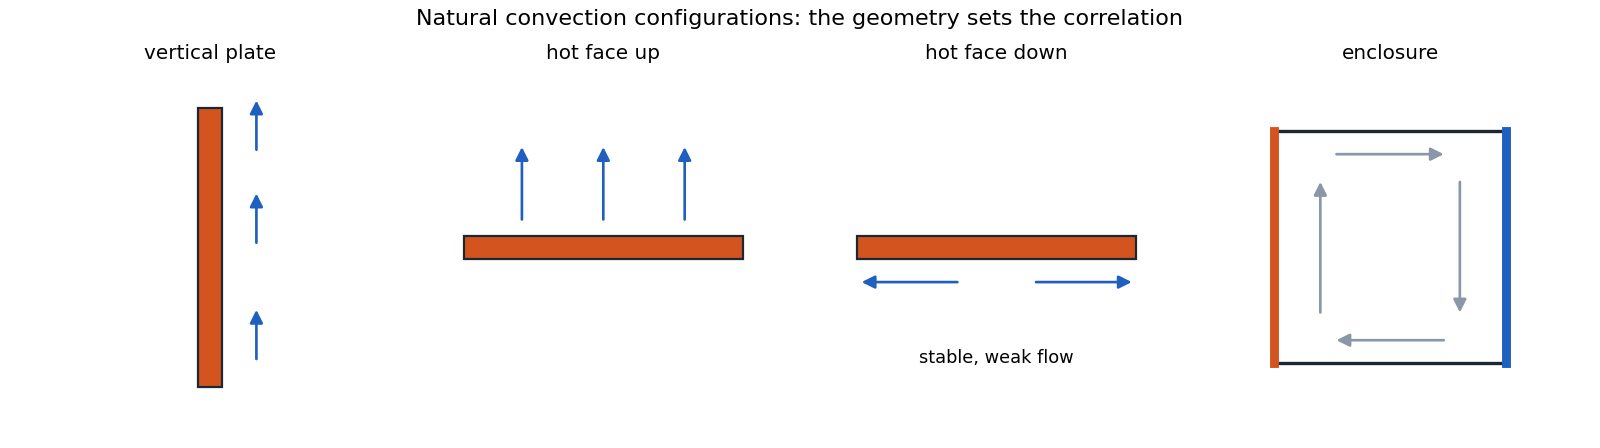
\includegraphics[width=0.75\linewidth]{pics/natural_convection_big_picture.png}
    \caption{Natural Convection Configurations}
\end{figure}
%%%%%%%%%%%%%%%%%%%%%%%%%%%%%%%%%%%%%%%%%%%%%%%%%%%%%%%%%%%
\subsection*{Boundary Layers in Natural Convection}
\addcontentsline{toc}{subsection}{Boundary Layers in Natural Convection}
%%%%%%%%%%%%%%%%%%%%%%%%%%%%%%%%%%%%%%%%%%%%%%%%%%%%%%%%%%%
In natural convection, the development of velocity and thermal boundary layers differs from forced convection:

\begin{itemize}
    \item In forced convection, the velocity boundary layer develops first, and the thermal boundary layer develops within it
    \item In natural convection, fluid motion is caused by temperature differences, so the thermal boundary layer initiates the velocity boundary layer
    \item For most fluids with Prandtl numbers near 1 (like air and water), the velocity and thermal boundary layers are of similar thickness
    \item For fluids with very high Prandtl numbers (like oils), the velocity boundary layer can be much thicker than the thermal boundary layer
\end{itemize}
%

\begin{wrapfigure}{R}{0.35\textwidth}
\centering
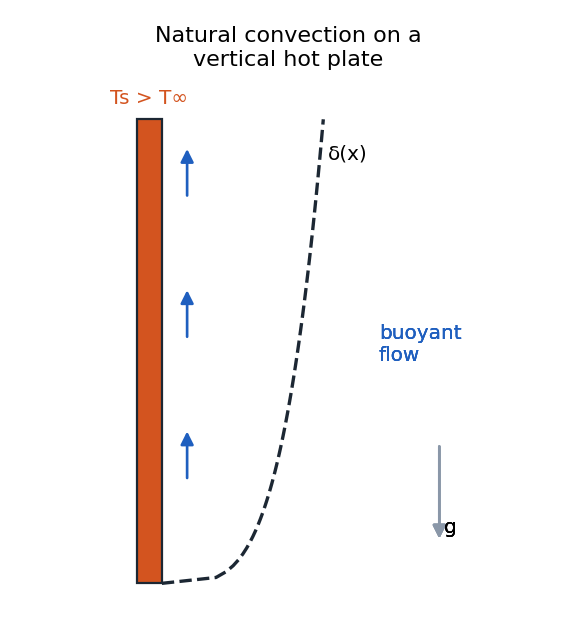
\includegraphics[width=0.7\linewidth]{pics/natural_convection.png}
\caption{figure}{$\delta$ and $\delta_t$ profile in natural convection.}
\end{wrapfigure}%
The velocity profile in natural convection is also distinctive:
    \begin{itemize}
        \item The fluid velocity is zero at the wall (no-slip condition)
        \item The velocity reaches a maximum within the boundary layer
        \item The velocity decreases to zero in the quiescent fluid outside the boundary layer
    \end{itemize}
This contrasts with forced convection, where the velocity asymptotically approaches the free stream velocity.
\[\]
\[\]
%%%%%%%%%%%%%%%%%%
\paragraph{Volumetric Thermal Expansion Coefficient: } This coefficient $\beta$ is used to relate the local density difference to the local temperature difference:
\[
    \beta=-\left.\frac{1}{\rho} \frac{\partial \rho}{\partial T}\right|_{p=\mathrm{constant}}
\]
    For ideal gases, $\beta = \frac{1}{T ~[\text{K}]}$ where $T$ is absolute temperature.
%%%%%

\paragraph{Boussinesq Approximation:} It assumes:
\begin{itemize}
    \item Neglect all other temperature-dependent property effects in the governing equations
    \item Density variation is approximated linearly with temperature:
    \[
        \beta \approx-\frac{1}{\rho} \frac{\left(\rho_{\infty}-\rho\right)}{\left(T_{\infty}-T\right)} \quad \Rightarrow \quad\left(\rho_{\infty}-\rho\right) \approx \rho \beta\left(T-T_{\infty}\right)
    \]

\end{itemize}

%%%%%%%%%%%%%%%%%%%%%%%%%%%%%%%%%%%%%%%%%%%%%%%%%%%%%%%%%%%
\subsection*{Natural Convection on Vertical Flat Plate}
\addcontentsline{toc}{subsection}{Natural Convection on Vertical Flat Plate}
%%%%%%%%%%%%%%%%%%%%%%%%%%%%%%%%%%%%%%%%%%%%%%%%%%%%%%%%%%%
\paragraph{Governing equations:}
\begin{enumerate}[(i)]
    \item Continuity equation:
    \[
        \frac{\partial u}{\partial x}+\frac{\partial v}{\partial y}=0
    \]
    %
    \item Momentum equation with buoyancy term:
    \textbf{}
    
    $x$-direction: 
    \[  
        \begin{aligned}
        & u \frac{\partial u}{\partial x}+v \frac{\partial u}{\partial y}= -\frac{1}{\rho} \overbrace{\frac{\partial P}{\partial x}}^{\rho_\infty g} - g +v \frac{\partial^2 u}{\partial y^2}
        \\[0.5em]
        &u \frac{\partial u}{\partial x}+v \frac{\partial u}{\partial y}=\frac{\left(\rho_{\infty}-\rho\right)}{\rho} g+v \frac{\partial^2 u}{\partial y^2}
        \\[0.5em]
        & u \frac{\partial u}{\partial x}+v \frac{\partial u}{\partial y}=g \beta\left(T-T_{\infty}\right)+v \frac{\partial^2 u}{\partial y^2}
        \end{aligned}
    \]
    \textbf{}
    
    $y$-direction: 
    \[
            0 = \frac{\partial P}{\partial y}
    \]
    %
    \item Energy equation:
    \[
        u \frac{\partial T}{\partial x}+v \frac{\partial T}{\partial y}=\alpha \frac{\partial^2 T}{\partial y^2}
    \]
\end{enumerate}
%
This can be solved using similarity method and
\[
    \eta=\frac{y}{x}\left(\frac{\mathrm{Gr}_x}{4}\right)^{1 / 4}
\]
%
\begin{figure}[H]
    \centering
    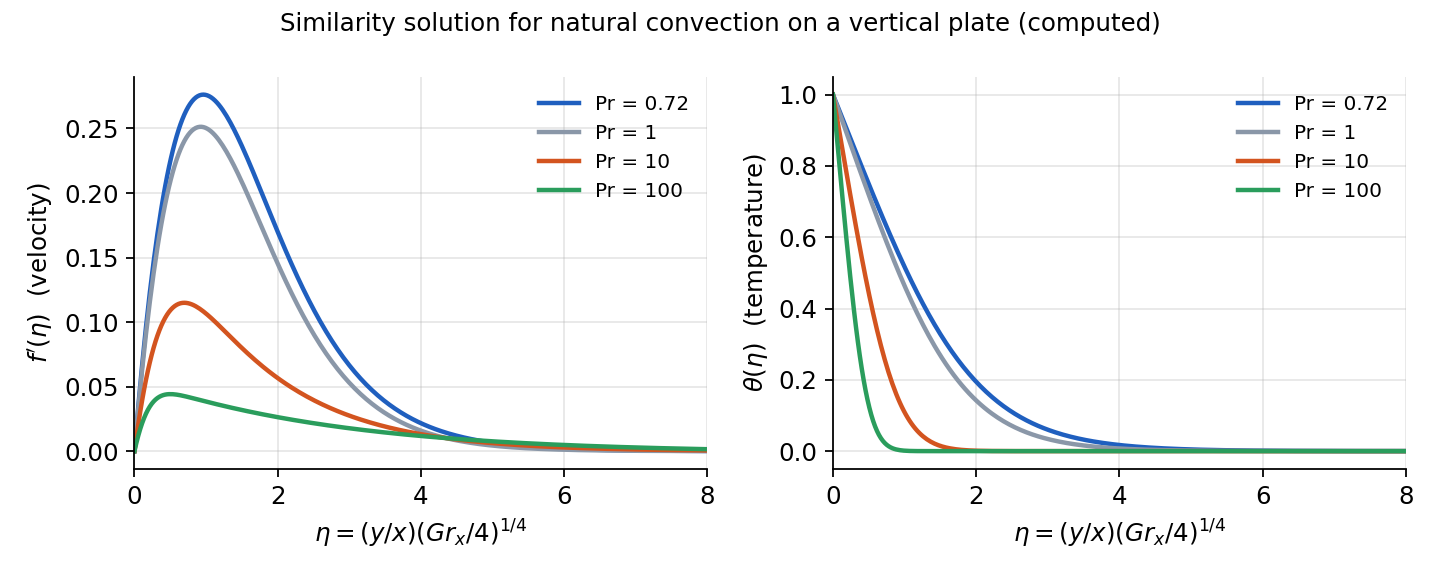
\includegraphics[width=0.65\linewidth]{pics/natural_convection_similarity.png}
    \caption{Similarity approach solution for natural convection in vertical flat plate.}
\end{figure}
%%%%%%%%%%%%%%%%%%%%%%%%%%%%%%%%%%%%%%%%%%%%%%%%%%%%%%%%%%%
\subsection*{Grashof and Rayleigh Dimensionless Numbers}
\addcontentsline{toc}{subsection}{Grashof and Rayleigh Dimensionless Numbers}
%%%%%%%%%%%%%%%%%%%%%%%%%%%%%%%%%%%%%%%%%%%%%%%%%%%%%%%%%%%
Natural convection problems introduce new dimensionless parameters:
\begin{definition}
\paragraph{Grashof Number}

The Grashof number represents the ratio of buoyancy forces to viscous forces:
\[
    \text{Gr}_L = \frac{g\beta(T_s-T_\infty)L^3}{\nu^2}
\]
\end{definition}

This parameter plays a role in natural convection similar to the Reynolds number in forced convection.
%
\begin{definition}
\paragraph{Rayleigh Number}

The Rayleigh number is the product of the Grashof and Prandtl numbers:
\[
    \text{Ra}_L = \text{Gr}_L \cdot \text{Pr} = \frac{g\beta(T_s-T_\infty)L^3}{\nu\alpha}
\]
\end{definition}
%%%%%%%%%%%%%%%%%%%%%%%%%%%%%%%%%%%%%%%%%%%%%%%%%%%%%%%%%%%
This parameter determines the nature of the flow and heat transfer in natural convection.

%%%%%%%%%%%%%%%%%%%%%%%%%%%%%%%%%%%%%%%%%%%%%%%%%%%%%%%%%%%%%%
\subsection*{Nusselt Number for Vertical Flat Plate}
\addcontentsline{toc}{subsection}{Nusselt Number for Vertical Flat Plate}
%%%%%%%%%%%%%%%%%%%%%%%%%%%%%%%%%%%%%%%%%%%%%%%%%%%%%%%%%%%%%%
Recall that the heat flux at the surface is by conduction
\[
    q_s^{\prime \prime}=-\left.k_f \frac{\partial T}{\partial y}\right|_{y=0}=-\left.\frac{k_f}{x}\left(T_s-T_{\infty}\right)\left(\frac{\mathrm{Gr}_x}{4}\right)^{1 / 4} \frac{d T^*}{d \eta}\right|_{\eta=0}
\]
\begin{definition}
 The Nusselt number then becomes
\[
    \mathrm{Nu}_x=\frac{h x}{k_f}=\frac{q_s^{\prime \prime}}{\left(T_s-T_{\infty}\right)} \frac{x}{k_f}=-\left.\left(\frac{\mathrm{Gr}_x}{4}\right)^{1 / 4} \frac{d T^*}{d \eta}\right|_{\eta=0}
\]
From the temperature profile solution
\[
    -\left.\frac{d T^*}{d \eta}\right|_{\eta=0}=f(\operatorname{Pr}) \approx \frac{0.75 \operatorname{Pr}^{1 / 2}}{\left(0.609+1.221 \operatorname{Pr}^{1 / 2}+1.238 \operatorname{Pr}\right)^{1 / 4}}
\]   
%
Therefore
\[
    h=\frac{q_s{ }^{\prime \prime}}{\left(T_s-T_{\infty}\right)}=\frac{k_f}{x}\left(\frac{\mathrm{Gr}_x}{4}\right)^{1 / 4} f(\operatorname{Pr})
\]
\end{definition}
%
\paragraph{Average Nusselt Numbers and h:} 
\[
    \bar{h}=\frac{1}{L} \int_0^L h d x=\frac{k_f}{L}\left(\frac{g \beta\left(T_S-T_{\infty}\right)}{4 v^2}\right)^{1 / 4} f(\operatorname{Pr}) \int_0^L \frac{1}{x^{1 / 4}} d x
\]
It can be shown that
\[
    \bar{h}=\frac{4}{3} h \Rightarrow \overline{\mathrm{Nu}}_L=\frac{4}{3} \mathrm{Nu}_L
\]
%%%%%%%%%%%%%%%%%%%%%%%%%%%%%%%%%%%%%%%%%%%%%%%%%%%%%%%%%%%%%%
\subsection*{Nusselt Number Empirical Correlations}
\addcontentsline{toc}{subsection}{Nusselt Number Empirical Correlations}
%%%%%%%%%%%%%%%%%%%%%%%%%%%%%%%%%%%%%%%%%%%%%%%%%%%%%%%%%%%%%%
For a vertical plate, critical Rayleigh number is $\mathrm{Ra}_{L,c} = 10^9$. Beyond this number, the flow is turbulent. Here are some useful formula for flat plate:

\begin{definition}
Nusselt number in free convection for vertical flat plates:

\[
    \overline{\mathrm{Nu}}_L=C \cdot \mathrm{Ra}_L^n : \quad
    \left\{
    \begin{array}{ccc}
        \text {Laminar flow: } & n=1 / 4, C=0.59 & \left(10^4<\mathrm{Ra}_L<10^9\right) 
        \\[1.5em]
        \text {Turbulent flow: } &n=1 / 3, C=0.10 & \left(\operatorname{Ra}_L>10^9\right)
    \end{array}\right.
\]

%
Alternatively, the \textit{Churchill} and \textit{Chu} correlation for the entire range of laminar and turbulent flow:
\[
    \overline{\mathrm{Nu}}_L=\left(0.825+\frac{0.378 \mathrm{Ra}_L^{1 / 6}}{\left[1+(0.492 / \mathrm{Pr})^{9 / 16}\right]^{8 / 27}}\right)^2
\]
\end{definition}


For horizontal plates and other geometries, specific correlations are available in heat transfer references.

When evaluating fluid properties, the film temperature should be used:
\[
T_f = \frac{T_s + T_\infty}{2}
\]
%
\begin{definition}
    For long horizotnal cylinder we have:
    \[
    \overline{N u}_D=\frac{\bar{h} D}{k}=C \operatorname{R a_D}^n
    \]
    where $C$ and $n$ can be calculated using the table below:
    \[
        \begin{array}{llc}
        \operatorname{\boldsymbol{R} \boldsymbol{a}_{\boldsymbol{D}}} & \boldsymbol{C} & \boldsymbol{n} \\
        \hline 10^{-10}-10^{-2} & 0.675 & 0.058 \\
        10^{-2}-10^2 & 1.02 & 0.148 \\
        10^2-10^4 & 0.850 & 0.188 \\
        10^4-10^7 & 0.480 & 0.250 \\
        10^7-10^{12} & 0.125 & 0.333 \\
        \hline
        \end{array}
    \]
\end{definition}



%%%%%%%%%%%%%%%%%%%%%%%%%%%%%%%%%%%%%%%%%%%%%%%%%%%%
\subsection*{Combined Forced and Natural Convection}
\addcontentsline{toc}{subsection}{Combined Forced and Natural Convection}
%%%%%%%%%%%%%%%%%%%%%%%%%%%%%%%%%%%%%%%%%%%%%%%%%%%%
In many real situations, both forced and natural convection effects are present. The relative importance is determined by comparing the Grashof and Reynolds numbers:

\begin{itemize}
    \item $\text{Gr}_L/\text{Re}_L^2 \ll 1$: Forced convection dominates
    \item $\text{Gr}_L/\text{Re}_L^2 \gg 1$: Natural convection dominates
    \item $\text{Gr}_L/\text{Re}_L^2 \approx 1$: Both mechanisms are significant
\end{itemize}

For the combined case, the general approach is to calculate both the forced convection Nusselt number ($\text{Nu}_{\text{forced}}$) and the natural convection Nusselt number ($\text{Nu}_{\text{natural}}$), then combine them using an appropriate correlation:
\[
\text{Nu} = (\text{Nu}_{\text{forced}}^3 + \text{Nu}_{\text{natural}}^3)^{1/3}
\]

This approach accounts for both mechanisms and provides a smooth transition between the limiting cases.

\subsection*{Applications of Natural Convection}
\addcontentsline{toc}{subsection}{Applications of Natural Convection}

Natural convection is important in many applications:
\begin{itemize}
    \item Cooling of electronic components
    \item HVAC systems and building ventilation
    \item Solar collectors and thermal energy storage
    \item Food processing and preservation
    \item Environmental flows in the atmosphere and oceans
    \item Passive cooling systems in nuclear reactors
\end{itemize}

While natural convection typically provides lower heat transfer coefficients than forced convection (2-25 W/m²K vs. 25-250 W/m²K), it requires no external power for fluid motion, making it desirable for passive cooling systems and energy-efficient designs.